\chapter{Eléments finis de Lagrange}
%
%
\noindent
On va présenter dans ce chapitre le type le plus simple et le plus classique
d'éléments finis.
%
%
\section{Unisolvance}
%
\noindent
%
\begin{definition}
  \label{def:22}
  Soit $\Sigma=\{ a_1,\ldots,a_N\}$ un ensemble de $N$ points distincts de
  $\RR^n$. Soit $P$ un espace vectoriel de dimension finie de fonctions de
  $\RR^n$ à valeurs dans \RR. On dit que $\Sigma$ est $P$-unisolvant ssi
  pour tous réels $\alpha_1,\ldots,\alpha_N$, il existe un unique
  élément $p$ de $P$ tel que $p(a_i)=\alpha_i,\; i=1,\ldots,N$.
\end{definition}

Ceci revient à dire que la fonction :
\begin{equation}
\label{eq:26}
\begin{array}{rcl}
{\cal L} : P & \longrightarrow & \RR^N\\
p & \longrightarrow & (p(a_1),\ldots,p(a_N))
\end{array}
\end{equation}
est bijective.\saut
%
%
En pratique, on montrera que $\Sigma$ est $P$-unisolvant en vérifiant que
dim $P=$ Card $\Sigma$, puis en montrant l'injectivité ou la surjectivité
de ${\cal L}$.
%
L'injectivité de ${\cal L}$ se démontre en établissant que la seule
fonction de $P$ s'annulant sur tous les points de $\Sigma$ est la fonction
nulle.
%
La surjectivité de ${\cal L}$ se démontre en exhibant une famille
$p_1,\ldots,p_N$ d'éléments de $P$ tels que $p_i(a_j)=\delta_{ij}$, c'est
à dire un antécédent pour ${\cal L}$ de la base canonique de $\RR^N$. En
effet, étant donnés des réels $\alpha_1,\ldots,\alpha_N$, la fonction
$\ds{p=\sum_{i=1}^N \alpha_i p_i}$ vérifie alors $p(a_j)=\alpha_j,\;
j=1,\ldots,N$.
%
%
\section{Elément fini de Lagrange}
\label{sec:lagrange}
\noindent
%
%
\begin{definition}
  Un {\bf élément fini de Lagrange} est un triplet $(K,\Sigma,P)$ tel que
  \begin{itemize}
  \item $K$ est un élément géométrique de $\RR^n$ ($n=$ 1, 2 ou 3),
    compact, connexe, et d'intérieur non vide.
%
  \item $\Sigma=\{a_1,\ldots,a_N\}$ est un ensemble fini de $N$ points
    distincts de $K$.
%
  \item $P$ est un espace vectoriel de dimension finie de fonctions réelles
    définies sur $K$, et tel que $\Sigma$ soit $P$-unisolvant (donc dim $P =
    N$).
  \end{itemize}\label{def:25}
\end{definition}

%
\begin{definition}
  Soit $(K,\Sigma,P)$ un élément fini de Lagrange. On appelle {\bf
  fonctions de base locales} de l'élément les $N$ fonctions $p_i$
  ($i=1,\ldots,N$) de $P$ telles que
  \begin{equation}
    \label{eq:27}
    p_i(a_j)=\delta_{ij}\qquad 1\le i,j \le N.
  \end{equation}
  \label{def:26}
\end{definition}
%
On vérifie aisément que $(p_1,\ldots,p_N)$ ainsi définie forme bien une
base de $P$.
%
%
\begin{definition}
  On appelle {\bf opérateur de interpolation} (ou encore $P-$interpolation)
  sur $\Sigma$ l'opérateur $\pi_K$ qui, à toute fonction $v$ définie sur
  $K$, associe la fonction $\pi_K v$ de $P$ définie par $\ds{\pi_K v =
  \sum_{i=1}^N v(a_i)\, p_i}$. $\pi_K v$ est donc l'unique élément de $P$
  qui prend les mêmes valeurs que $v$ sur les points de
  $\Sigma$.\label{def:27}
\end{definition}

%
%
\section{Exemples d'éléments finis de Lagrange}
%
\subsection{Espaces de polyn\^omes}
\noindent
%
On notera $\Pk$ l'espace vectoriel des polyn\^omes de degré total inférieur ou égal à $k$.
%
\begin{itemize}
\item Sur \RR, $\Pk=\hbox{Vect} \{ 1,X,\ldots, X^k\}\quad$ et dim $\Pk=k+1$.
\item Sur \RR$^2$, $\Pk=\hbox{Vect} \{ X^i Y^j ; 0\le i+j \le k\}\quad$ et dim $\ds{ \Pk=\frac{(k+1)(k+2)}{2}}$.
\item Sur \RR$^3$, $\Pk=\hbox{Vect} \{ X^i Y^j Z^l ; 0\le i+j+l \le k\}\quad$ et dim $\ds{ \Pk=\frac{(k+1)(k+2)(k+3)}{6}}$.
\end{itemize}
%
On notera $\Qk$ l'espace vectoriel des polyn\^omes de degré inférieur ou égal à $k$ par rapport à chaque variable.
%
\begin{itemize}
\item Sur \RR, $\Qk=\Pk$.
\item Sur \RR$^2$, $\Qk=\hbox{Vect} \{ X^i Y^j ; 0\le i,j \le k\}\quad$ et dim $\ds{ \Qk=(k+1)^2}$.
\item Sur \RR$^3$, $\Qk=\hbox{Vect} \{ X^i Y^j Z^l ; 0\le i,j,l \le k\}\quad$ et dim $\ds{ \Qk=(k+1)^3}$.
\end{itemize}
%
%
\subsection{Exemples 1-D}
\label{par:ex1d}
%
\subsubsection{Elément $P_1$}
\begin{itemize}
\item $K=[a,b]$
\item $\Sigma=\{a,b\}$
\item $P=\Pk[1]$
\end{itemize}
%
\subsubsection{Elément $P_2$}
\begin{itemize}
\item $K=[a,b]$
\item $\ds{\Sigma=\{a,\frac{a+b}{2},b\}}$
\item $P=\Pk[2]$
\end{itemize}
%
%
\subsubsection{Elément $\Pk$}
\begin{itemize}
\item $K=[a,b]$
\item $\ds{\Sigma=\{a+i\,\frac{b-a}{m},\quad i=0,\ldots,k\}}$
\item $P=\Pk$
\end{itemize}
%
%
\subsection{Exemples 2-D triangulaires}
%
%
\subsubsection{Elément $\Pk[1]$}
\begin{itemize}
\item $K$=triangle de sommets $a_1, a_2, a_3$
\item $\Sigma=\{a_1,a_2,a_3\}$
\item $P=\Pk[1]$
\end{itemize}
%
Les fonctions de base sont définies par $p_i(a_j)=\delta_{ij}$. Ce sont donc
les coordonnées barycentriques : $p_i=\lambda_i$ (cf annexe \ref{ch:bary}).
%
%
\subsubsection{Elément $\Pk[2]$}
\begin{itemize}
\item $K$=triangle de sommets $a_1, a_2, a_3$
\item $\Sigma=\{a_1,a_2,a_3, a_{12}, a_{13}, a_{23}\}$,\/ o\`u $\ds{a_{ij}=\frac{a_i+a_j}{2}}$.
\item $P=\Pk[2]$
\end{itemize}
%
Les fonctions de base sont $p_i=\lambda_i (2\lambda_i -1)$ et
$p_{ij}=4\lambda_i\lambda_j$. Un exemple de calcul de ces fonctions de base
est donné en annexe \ref{ch:bary}.
%
\begin{figure}[h]
\begin{center}
\includegraphics[width=0.95\linewidth]{FIG/elements-2D.jpg}
%\vspace*{6.5 cm}
\caption{Eléments finis triangulaire $P_1$, triangulaire $P_2$ et rectangulaire $Q_1$}
\end{center}
\end{figure}
%
%
\subsection{Exemples 2-D rectangulaires}
%
\subsubsection{Elément $\Qk[1]$}
\begin{itemize}
\item $K$=rectangle de sommets $a_1, a_2, a_3, a_4$, de c\^otés parallèles aux axes
\item $\Sigma=\{a_1,a_2,a_3,a_4\}$
\item $P=\Qk[1]$
\end{itemize}
%
Les fonctions de base sont
$\ds{p_i(X,Y)=\frac{(X-x_j)(Y-y_j)}{(x_i-x_j)(y_i-y_j)}}$, o\`u $(x_i,y_i)$
sont les coordonnées de $a_i$, et o\`u $a_j$, de coordonnées $(x_j,y_j)$
est le coin opposé à $a_i$.
%
%%
\subsection{Exemples 3-D}
%
%
%
\subsubsection{Elément tétraèdrique $\Pk[1]$}
\begin{itemize}
\item $K$=tétraèdre de sommets $a_1, a_2, a_3, a_4$
\item $\Sigma=\{a_1,a_2,a_3, a_4\}$
\item $P=\Pk[1]$
\end{itemize}
%
%
\subsubsection{Elément tétraèdrique $\Pk[2]$}
\begin{itemize}
\item $K$=tétraèdre de sommets $a_1, a_2, a_3, a_4$
\item $\ds{ \Sigma=\{a_i\}_{1\le i\le 4} \cup \{a_{ij}\}_{1\le i < j \le 4} }$
\item $P=\Pk[2]$
\end{itemize}
%
Les fonctions de base sont $p_i=\lambda_i (2\lambda_i -1)$ et $p_{ij}=4\lambda_i\lambda_j$.
%
%
\subsubsection{Elément parallélépipèdique $Q_1$}
\begin{itemize}
\item $K$=parallélépipède de sommets $a_1, \ldots , a_8$ de c\^otés parallèles aux axes
\item $\Sigma=\{a_i\}_{1\le i\le 8}$
\item $P=\Qk[1]$
\end{itemize}
%
%
\subsubsection{Elément prismatique}
\begin{itemize}
\item $K$=prisme droit de sommets $a_1, \ldots , a_6$
\item $\Sigma=\{a_i\}_{1\le i\le 6}$
\item $P=\{p(X,Y,Z)=(a+bX+cY)+Z(d+eX+fY), \;\; a,b,c,d,e,f \in \RR\}$
\end{itemize}
%
%
\begin{figure}[h]
\begin{center}
\includegraphics[width=0.95\linewidth]{FIG/elements-3D.jpg}
%\vspace*{6.5 cm}
\caption{Eléments finis tétraèdriques $P_1$ et $P_2$, parallélépipèdique $Q_1$, et prismatique}
\end{center}
\end{figure}
%
%
\section{Famille affine d'éléments finis}
\noindent
%
%
\begin{definition}
  Deux éléments finis $(\hat{K},\hat{\Sigma},\hat{P})$ et $(K,\Sigma,P)$
  sont {\bf affine-équivalents} ssi il existe une fonction affine $F$
  inversible ($F: \hat{x} \longrightarrow B\hat{x}+b$) telle que
  \begin{itemize}
  \item $K=F(\hat{K})$
  \item $a_i=F(\hat{a}_i) \qquad i=1,\ldots,N$
  \item $P=\{ \hat{p}\circ F^{-1} , \quad \hat{p}\in \hat{P} \}$
  \end{itemize}\label{def:28}
\end{definition}
%
\begin{remark}
  Si l'on est dans $\RR^n$, $B$ est donc une matrice $n\times n$ inversible,
  et $b$ est un vecteur de $\RR^n$.\label{rem:10}
\end{remark}

%
{\bf Propriété :} Soient $(\hat{K},\hat{\Sigma},\hat{P})$ et
$(K,\Sigma,P)$ deux éléments finis affine-équivalents, via une
transformation $F$. On note $\hat{p}_i \; (i=1,\ldots,N)$ les fonctions de
base locales de $\hat{K}$. Alors les fonctions de base locales de $K$ sont les
$p_i=\hat{p}_i\circ F^{-1}$.
%
\begin{definition}
  On appelle {\bf famille affine d'éléments finis} une famille
  d'éléments finis tous affine-équivalents à un même élément
  fini $(\hat{K},\hat{\Sigma},\hat{P})$, appelé {\bf élément de
  référence}.\label{def:29}
\end{definition}

%
D'un point de vue pratique, le fait de travailler avec une famille affine
d'éléments finis permet de ramener tous les calculs d'intégrales à des
calculs sur l'élément de référence.
%
Les éléments de référence sont :
\begin{itemize}
\item En 1-D : le segment $[0,1]$
\item En 2-D triangulaire : le triangle unité, de sommets $(0,0)$, $(0,1)$ et $(1,0)$.
\item En 2-D rectangulaire : le carré unité $[0,1]\times[0,1]$.
\item En 3-D tétraèdrique : le tétraèdre unité, de sommets $(0,0,0)$, $(1,0,0)$, $(0,1,0)$ et $(0,0,1)$.
\item En 3-D parallélépipèdique : le cube unité $[0,1]\times[0,1]\times[0,1]$.
\item En 3-D prismatique : le prisme unité de sommets $(0,0,0)$, $(0,1,0)$, $(1,0,0)$, et $(0,0,1)$, $(0,1,1)$, $(1,0,1)$.
\end{itemize}

%
%

\subsection{Maillages}
\label{sec:maillages}

Nous étendons ici aux dimension 2 et 3 les notions élémentaires de maillage
vues en 1D, voir la figure~\ref{fig:2}.

\begin{figure}[htbp]
  \centering
  \subfigure[2D]{\includegraphics[width=.45\linewidth]{contact2d-crop}}
  \subfigure[3D]{\includegraphics[width=.45\linewidth]{contact3d-crop}}
  \caption{Un maillage en 2D et en 3D}
  \label{fig:2}
\end{figure}

\begin{definition}
  \label{def:31}
  Un maillage est constituée d'une famille d'éléments(ou mailles ou cellules)
  $\{K_e\}_{e=1,...,N_e}$ où $N_e$ est le nombre d'éléments, nous noterons
  \begin{equation}
    \label{eq:32}
    \calTh = \{K_m\}_{m=1,...,N_e}
  \end{equation}
  avec
  \begin{equation}
    \label{eq:33}
    h=\max_{1\le e\le N_e} h_{K_e}
  \end{equation}
  et
  \begin{equation}
    \label{eq:34}
    h_{K_e}     = \diam(K_e) = \max_{x_1,x_2 \in K_e} \|x_1-x_2\|,\, e \in \{1,...,\Ne\}
  \end{equation}

\end{definition}

On travaille par la suite avec des familles de maillage et on les note
$\set{\mathcal{T}_h}_{h > 0}$.

\begin{definition}[Maillage Quasi-uniforme]
  On dira qu'une famille de maillage $\set{\mathcal{T}_h}_{h > 0}$ est
  \textrm{quasi-uniforme} s'il existe une constante $c$ telle que
  \begin{equation}
    \label{eq:35}
    \forall h,\ \forall K \in \calTh,\ h_K \geq c h
  \end{equation}
\end{definition}

\begin{remark}
  Cela veut dire que les élements sont tous de la même taille pour $h$
  donné.\label{rem:12}
\end{remark}

\subsection{Transformation géométrique}
\label{sec:transf-geom}

Un maillage est généré par
\begin{enumerate}
\item un \emph{élément de reference} noté $\hat{K}$
\item une famille de  \emph{transformations géométriques} mappant $\hat{K}$
  vers les éléments $K_e, e=1,\ldots,\Ne$ dans le maillage
\end{enumerate}

Nous supposerons que les transformations sont des $\mathcal{C}^1-$
diffeomorphismes \footnote{la transformation et son inverse sont
$\mathcal{C}^1$ et bijectives}

\begin{definition}
  \label{def:32}
  Pour une cellule $K \in \mathcal{T}_h$, on note $T_K$ la  transformation géométrique
  \begin{equation}
    \label{eq:36}
    T_K: \hat{K} \mapsto K
  \end{equation}
\end{definition}

Afin de spécifier la transformation géométrique, on  considère l'élément fini
de Lagrange, noté $(\hat{K},\hat{P}_{\mathrm{geo}},
\hat{\Sigma}_{\mathrm{geo}})$, tel que
  \begin{itemize}
  \item $\ngeo = \card{\hat{\Sigma}_{\mathrm{geo}}}$
  \item $\set{\hat{g}_1,\ldots,\hat{g}_{\ngeo}}$ les noeuds de $\hat{K}$
  \item $\set{\hat{\psi}_1,\ldots,\hat{\psi}_{\ngeo}}$ les fonctions de forme
  \end{itemize}

\begin{definition}[Élément fini géométrique]
  On dit que
  \begin{itemize}
  \item $(\hat{K},\hat{P}_{\mathrm{geo}}, \hat{\Sigma}_{\geo})$ est
    l'\emph{élément fini géométrique},
  \item $\set{\hat{g}_1,\ldots,\hat{g}_{\ngeo}}$ sont les  \emph{noeuds géométriques} et
  \item $\set{\hat{\psi}_1,\ldots,\hat{\psi}_{\ngeo}}$ sont les
    \emph{fonctions de formes géométriques}
  \end{itemize}
\end{definition}
\begin{figure}[htbp]
  \centering
  \centerline{\includegraphics[width=.5\linewidth]{pdfs/pena/py_figures/geomap_triangle}}
  \caption{Transformation géométrique associée à un triangle}
  \label{fig:3}
\end{figure}

Pour chaque $K \in \mathcal{T}_h$, on a un $\ngeo$-uplet
$\set{g^K_1,\ldots,g^K_\ngeo}$. La transformation géométrique est définie
comme suit
\begin{equation}
  \label{eq:37}
  T_K: \hat{x} \in \hat{K} \mapsto \sum_{i=1}^\ngeo\ g^K_i \hat{\psi}_i(\hat{x})
\end{equation}
et en particulier on a
\begin{equation}
  \label{eq:38}
  T_K(\hat{g}_i) = g^K_i, \quad \forall i \in \set{1,\ldots,\ngeo}
\end{equation}
\begin{remark}
  \label{rem:13}
  On a $T_K \in [\hat{P}_\geo(\hat{K})]^d$ et que  $\set{g^K_1,\ldots,g^K_\ngeo}$ sont les \emph{noeuds géométriques} de $K$.
\end{remark}

$T_K$ est un $\mathcal{C}^1$-diffeomorphism donc la \emph{numérotation} des noeuds
$\set{g^K_1,\ldots,g^K_\ngeo}$ doit être  \emph{compatible} avec les noeuds de
l'élément finit géométrique.

\begin{minipage}[l]{.3\linewidth}
\centerline{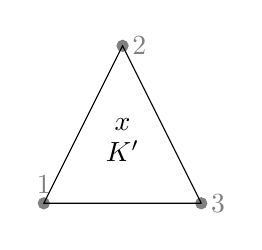
\begin{tikzpicture}
  \filldraw [gray] (2,0) circle (2pt) node [right] (a) {3}
  (1,2) circle (2pt) node[right] (b) {2}
  (0,0) circle (2pt) node[above] (c) {1};
  \node[] at (1,1) (x1) {$x$};
  \draw (2,0) -- (1,2) -- (0,0) -- (2,0);
  \node[] at (1,0.6666) {$K'$};
\end{tikzpicture}}
\centerline{Numérotation pas OK}
\end{minipage}
\begin{minipage}[c]{.3\linewidth}
\centerline{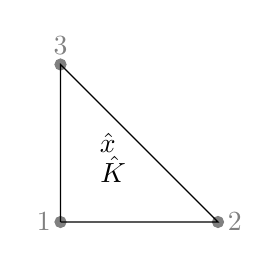
\begin{tikzpicture}
  \filldraw [gray] (-1,-1) circle (2pt) node [left] {1}
  (1,-1) circle (2pt) node[right] {2}
  (-1,1) circle (2pt) node[above] {3};
  \node[] at (-0.4,0) (hatx) {$\hat{x}$};
  \draw (-1,-1) -- ( 1,-1 ) -- (-1,1) --(-1,-1);
  \node[] at (-0.3333,-0.333) {$\hat{K}$};
\end{tikzpicture}}
\end{minipage}
\begin{minipage}[r]{.3\linewidth}
\centerline{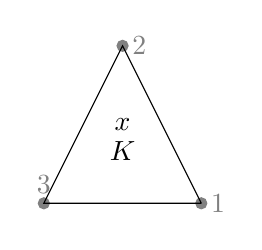
\begin{tikzpicture}
  \filldraw [gray] (2,0) circle (2pt) node [right] (a) {1}
  (1,2) circle (2pt) node[right] (b) {2}
  (0,0) circle (2pt) node[above] (c) {3};
  \node[] at (1,1) (x2) {$x$};
  \draw (2,0) -- (1,2) -- (0,0) -- (2,0);
  \node[] at (1,0.6666) {$K$};
\end{tikzpicture}}
\centerline{Numérotation OK}
\end{minipage}


\begin{tikzpicture}[overlay]
  \path[->] (hatx) edge [bend left] node[auto] {$T_K$}(x2);
  \path[->] (hatx) edge [bend right] node[auto] {$T_{K'}$}(x1);
\end{tikzpicture}

\begin{remark}
  \label{rem:15}
  La numérotation locale des entités géométriques dans \Feel \textbf{doit}
  être consistente avec la numérotation locale des générateurs de
  maillafe. voir
  \href{http://www.geuz.org/gmsh/doc/texinfo/gmsh.html#Node-ordering}{\color{blue}$\triangleright$~format
  de fichier Gmsh} pour une numérotation locale.
\end{remark}


Un cas particulier est la transformation géométrique affine

\begin{definition}[Maillage affine]
  \label{def:33}
  Quand toutes les  \emph{transformations géométriques} $\set{T_K}_{K \in
  \mathcal{T}_h}$ sont \emph{affines}, cela veut dire que pour tout $K \in
  \mathcal{T}_h$, il existe un  vecteur $b_K \in \R[d]$ et une matrice $J_K \in
  \R[{d,d}]$ tels que
  \begin{equation}
    \label{eq:39}
    T_K : \hat{x} \in \hat{K} \mapsto b_K + J_K \hat{x}  \in K
  \end{equation}
  On dit que le maillage est \emph{affine}.
\end{definition}
\begin{remark}[Exemple]
  \label{rem:16}
  Si l'élément fini géométrique est $(\hat{K},\poly{P}_1,\Sigma_\ngeo)$ alors
  les éléments $K$ sont soit des triangles soit des tétrahèdres.
\end{remark}

\begin{remark}[\Feel]
  \label{rem:17}
  \lstinline!Mesh<Simplex<d,1> >! ou \lstinline!Mesh<Simplex<d> >! est le type
  pour les maillages affines formés de simplexes dans $\R[d]$.
  \lstinline!1! indique l'ordre de l'\emph{élément fini géométrique} (here 1).
\end{remark}

\subsection{Quelques calculs avec la transformation géométrique}
\label{sec:quelq-calc-avec}

\subsubsection{Gradient, Inverse et Jacobien}
\label{sec:gradient-inverse-et}

On note $\xi$ un ensemble de  $n$ points dans $\hat{K}$ et on note $\nabla
T_K(\xi)$ le gradient de $T_K$ aux points $\xi$
\begin{equation}
  \label{eq:40}
  \nabla T_K( \xi )\ =\ \sum_{i=0}^{\ngeo}\ g^K_i\ \nabla \psi_i (\xi)
\end{equation}
et $B_K(\xi) = \nabla T_K^{-1}(\xi)$ l'inverse $\xi$
et finalement $J_K(\xi)$ le jacobien de $T_K$ en $\xi$
\begin{equation}
\label{eq:41}
J_K(\xi)\ =\ |\det( \nabla T_K(\xi) )|
\end{equation}

\subsubsection{Dérivation dans l'élément de référence}
\label{sec:deriv-dans-lelem}

Afin de dériver un polynome dans l'élément réel $K$, grâce à la transformation
géométrique et la règle de différentiation des fonctions composées, nous
dérivons seulement dans l'élément de référence $\hat{K}$.

Soit $f: K \mapsto \R[]$ et $\hat{f}: \hat{K} \mapsto \R[]$ telle
que $\hat{f} = f \circ T_K$
\begin{equation}
  \label{eq:42}
  \nabla f\ =\  \hat{\nabla} \underbrace{\hat{f}(\xi)}_{f \circ T_K(\xi)} B_K(\xi)
\end{equation}

en 2D, on a
\begin{equation}
  \label{eq:43}
  \nabla f(x) =
  \begin{pmatrix}
    \frac{\hat{\partial} \hat{f} (\xi)}{\partial \xi_1} & \frac{\hat{\partial} \hat{f} (\xi)}{\partial \xi_2}
  \end{pmatrix}
  \begin{pmatrix}
    B_{K_{11}}(\xi) & B_{K_{12}}(\xi)\\
    B_{K_{21}}(\xi) & B_{K_{22}}(\xi)\\
  \end{pmatrix}
\end{equation}
avec $x=T_K(\xi)$
% \end{block}

\subsubsection{Intégration dans l'élément de référence}
\label{sec:integr-dans-lelem}

De manière similaire, au lieu de calculer les intégrales sur l'élément réel
$K$, nous appliquons un changement de variables et calculons les intégrales
sur l'élément de réference $\hat{K}$.

Soit $f: K \mapsto \R[]$ et $\hat{f}: \hat{K} \mapsto \R[]$ telle que
 $\hat{f} = f \circ T_K$, et ${\bm F}: K \mapsto
\R[d]$ et ${\hat{\bm F}}: \hat{K} \mapsto \R[d]$ telle que
$\hat{{\bm F}} = {\bm F} \circ T_K$, on a alors les relations suivantes

\begin{equation}
  \label{eq:44}
  \int_{K} \ f\ dx\ =\ \int_{\hat{K}} f(T_K(\xi) ) J_K( \xi )\ d \xi \ =\ \int_{\hat{K}} \hat{f}(\xi) J_K( \xi )\ d \xi
\end{equation}
\begin{equation}
  \label{eq:45}
  \int_{K}\ \nabla f\ dx\ =\ \int_{\hat{K}} \Big(\hat{\nabla} \underbrace{\hat{f}(\xi)}_{f \circ T_K(\xi)} B_K(\xi)\Big) J_K( \xi )\ d \xi
\end{equation}
\begin{equation}
  \label{eq:46}
  \int_{\partial K}\ f( x )\ dx = \int_{\partial \hat{K}} \hat{f}(\xi)\  \| B_K(\xi) \ {\hat{\bm n}}(\xi) \|\ J_K( \xi )\ d \xi
\end{equation}
\begin{equation}
  \label{eq:47}
  \int_{\partial K}\ {\bm F}( x )\ \cdot\ {\bm n}(x) dx = \int_{\partial \hat{K}} {\hat{\bm F}}( \xi )\  \cdot \Big(B_K(\xi) \ {\hat{\bm n}}(\xi) \Big) \ J_K( \xi )\ d \xi
\end{equation}
où ${\bm n}(x)$ est la \emph{normale extérieure unitaire} à $\partial K$
évaluée en $x \in \partial K$, et ${\hat{\bm n}}(\xi)$ la normale unitaire extérieure
à  $\hat{K}$ évaluée en $\xi \in \partial \hat{K}$.

\begin{remark}
  \label{rem:18}
  \Feel effectue automatiquement pour vous les changements de variables dans
  les intégrales.
\end{remark}


\begin{definition}[Maillages conformes]
  \label{def:34}
  Un maillage est dit \emph{conforme} si l'intersection de deux éléments est
  soit vide, un sommet, une arête ou une face.
\end{definition}

\begin{minipage}[l]{.3\linewidth}
  \centerline{
  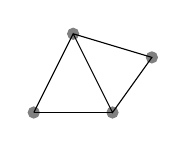
\begin{tikzpicture}
    \filldraw [gray] (0,0) circle (2pt)
    (0.5,1) circle (2pt)
    (1,0) circle (2pt)
    (1.5,0.7) circle (2pt);
    \draw (0,0) -- (0.5,1) -- (1,0) -- (1.5,0.7) -- (0.5,1);
    \draw (0,0) -- (1,0);
  \end{tikzpicture}}
  \centerline{Conforme}
\end{minipage}
\begin{minipage}[c]{.3\linewidth}
  \centerline{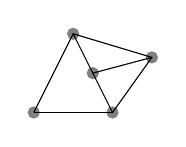
\begin{tikzpicture}
    \filldraw [gray] (0,0) circle (2pt)
    (0.5,1) circle (2pt)
    (1,0) circle (2pt)
    (1.5,0.7) circle (2pt)
    (0.75,0.5) circle (2pt)
    ;
    \draw (0,0) -- (0.5,1) -- (1,0) -- (1.5,0.7) -- (0.5,1);
    \draw (0,0) -- (1,0);
    \draw (1.5,0.7) -- (0.75,0.5);
  \end{tikzpicture}}
  \centerline{Pas conforme}
\end{minipage}

\begin{remark}[\Feel]
  \label{rem:19}
  On ne manipule que des maillages conformes dans le cours mais \Feel peut
  traiter des maillages non-conformes par exemple dans le contexte de méthode
  de décomposition de domaines.
\end{remark}


\subsection{Génération des éléments finis de Lagrange}


\begin{itemize}
\item Soit $\mathcal{T}_h$ un maillage généré par $(\hat{K},
  \hat{P}_{\mathrm{geo}}, \hat{\Sigma}_{\mathrm{geo}})$
\item une cellule $K \in \mathcal{T}_h$ est alors l'image de  $\hat{K}$ par la
  transformation géométrique $T_K$ défini par \eqref{eq:23}
\end{itemize}

L'objectif à présent est de générer la famillage l'éléments finis de Lagrange
grâce à l'élément fini de référence $(\hat{K},\hat{P}, \hat{\Sigma})$
\begin{equation}
  \label{eq:28}
  \{(K,P_K,\Sigma_K)\}_{K \in \mathcal{T}_h}
\end{equation}
\begin{itemize}
\item on note $\{\hat{x}_1,...,\hat{x}_{\nf}\}$ les noeuds de l'élément fini
\item on note $\{\hat{\Psi}_1,...,\hat{\Psi}_{\nf}\}$ les fonctions de forme
  élément fini
\end{itemize}

\begin{proposition}
  \label{prop:6}
  \begin{itemize}
  \item Soit $K \in \mathcal{T}_h$ et $P_K=\{\hat{p} \circ T_K^{-1}; \hat{p} \in \hat{P}\}$
  \item Pour tout $i \in \{1,...,\nf\}$, on pose $x_{K,i} = T_K(\hat{x}_i)$
  \item $\Sigma_K$ est l'ensemble des \emph{degrés de liberté} associé à $\{x_{K,1},...,x_{K,\nf}\}$
  \end{itemize}
  Alors $(K,P_K,\Sigma_K)$ est un \emph{élément fini de Lagrange}.
  Les  \emph{fonctions de forme} sont définies de la fa\c {c}on suivante
  \begin{equation}
    \label{eq:49}
    \Psi_{K,i} = \hat{\Psi}_i \circ T_K^{-1}, \quad i=1,...,\nf
  \end{equation}
  et \Ilag{K}  l'\emph{opérateur d'interpolation local}  comme
    \begin{equation}
      \label{eq:50}
      \Ilag{K}: v \in \mathcal{C}^0(K) \mapsto \sum_{i=1}^\nf\ v(x_{K,i})\ \Psi_{K,i}\
      \in P_K
    \end{equation}
    Une propriété importante de \Ilag{K} est que
    \begin{equation}
      \label{eq:51}
      \forall v \in \mathcal{C}^0(K),\quad \Ilag{K}( v \circ T_K ) =
      \Ilag{K}( v ) \circ T_K.
    \end{equation}
  \end{proposition}

  \begin{theorem}[Propriété de l'interpolateur local]
    \label{thr:14}
    \begin{itemize}
    \item Soit $T_K$ une transformation affine
    \item Soit $\mathbb{P}_k \subset \hat{P}$ et $k+1 > \frac{d}{2}$
    \item Soit $h_K$ le diamètre de $K$ et $\rho_K$ le diamètre de la plus
      grande boule      inscrite  dans $K$ et  $\omega_K = \frac{h_K}{\rho_K}$
    \end{itemize}
    Alors il existe une constante $c$ independente de $K$ telle que $\forall v \in
    H^{k+1}(K)$ et pour tout $m \in \{0,...,k+1\}$,
    \begin{equation}
      \label{eq:32}
      |v - \Ilag{K}(v)|_{m,K} \leq  c h^{k+1-m} \omega_K^m |v|_{k+1,K}
    \end{equation}
  \end{theorem}
  \begin{remark}
    \label{rem:20}
    \begin{itemize}
    \item $\omega_K$ devrait être aussi proche de $1$ que possible
    \item La deuxième hypothèse technique permettant d'assurer que $H^{k+1}(K) \subset
      C^0(K)$.
    \item on obtient des résultats similaires si $v$ n'est pas suffisamment régulière
    \end{itemize}

  \end{remark}

  \begin{definition}[Espaces $H^1$ conformes]
    \label{def:35}
    Un espace vectoriel $V_h$ de fonctions définies sur un domaine $\Omega_h$
    est dit être $H^1$-conforme si $V_h \subset H^1(\Omega_h)$
  \end{definition}
  Afin de construire un tel espace on introduit tout d'abord
    \begin{equation}
      \label{eq:52}
      W_h = \{v_h \in L_2(\Omega_h); \forall K \in \mathcal{T}_h, v_h|_K \in P_K\}
    \end{equation}
    mais ce n'est pas suffisant: \emph{les fonctions $W_h$ peuvent avoir des
    sauts entre les éléments du maillage}. Nous avons donc besoin d'assurer la
    \emph{continuité} de ces fonctions
    \begin{equation}
      \label{eq:53}
      V_h = W_h \cap C^0(\Omega_h) = \{ v_h \in W_h; \forall F \in
      \mathcal{F}^i_h. \jump{v_h}_F = 0\}
    \end{equation}
    Concernant l'implémentation, nous avons besoin de d'indentifier les
    \emph{degrés de liberté communs entre les éléments} quand nous construisons
    la tables des degrés de liberté.

    Voici deux exemples d'espace $H^1$-conforme
    \begin{equation}
      \label{eq:54}
      P^k_{c,h} = \{ v_h \in C^0(\Omega_h); \forall K \in \mathcal{T}_h, v_h
      \circ T_K \in \mathbb{P}_k\}
    \end{equation}
    \begin{equation}
      \label{eq:55}
      Q^k_{c,h} = \{ v_h \in C^0(\Omega_h); \forall K \in \mathcal{T}_h, v_h
      \circ T_K \in \mathbb{Q}_k\}
    \end{equation}

    \subsection{Projections orthogonales}
    \label{sec:proj-orth}

    \begin{definition}{Projection Orthogonale}
      \label{def:36}
      On note
      \begin{eqnarray}
        \label{eq:56}
        \Pi^{0,k}_{c,h} : L_2(\Omega) \rightarrow P^k_{c,h}\\
        \Pi^{1,k}_{c,h} : H^1(\Omega) \rightarrow P^k_{c,h}
      \end{eqnarray}
      associés respectivement aux produits scalaires
      $(u,v)_{0,\Omega} = \int_\Omega u v$ and $(u,v)_{1,\Omega} = \int_\Omega u
      v + \int_\Omega \nabla u \cdot \nabla v$
      On a pour $l=1,...,k$ et si $v \in H^{l+1}(\Omega)$
      \begin{eqnarray}
        \label{eq:57}
        \|v - \Pi^{0,k}_{c,h}(v)\|_{0,\Omega} &\leq c h^{l+1} |v|_{k+1,\Omega} \\
        \|v - \Pi^{1,k}_{c,h}(v)\|_{1,\Omega} &\leq c h^{l} |v|_{k+1,\Omega}
      \end{eqnarray}
    \end{definition}

    Pour calculer  $\Pi^{0,k}_{c,h}$ et $\Pi^{1,k}_{c,h}$ on a besoin de
    résoudre les     problèmes
    \begin{problem}[Projection $L_2$]
      \label{prob:3}
      Soit $v$ une fonction de $L_2$, calculer $\Pi^{0,k}_{c,h}(v) \in
      P^k_{c,h}$ tel que $\forall v_h \in P^k_{c,h}$ on a
      \begin{equation}
        \label{eq:58}
        (\Pi^{0,k}_{c,h}(v), v_h)_{0,\Omega} = (v, v_h)_{0,\Omega}
      \end{equation}
\end{problem}

\begin{problem}[Projection $H^1$]
  \label{prob:4}
  Soit $v$ une fonction de $H^1$, calculer $\Pi^{1,k}_{c,h}(v) \in
  P^k_{c,h}$ tel que $\forall v_h \in P^k_{c,h}$ on a
  \begin{equation}
    \label{eq:59}
    (\Pi^{1,k}_{c,h}(v), v_h)_{1,\Omega} = (v, v_h)_{1,\Omega}
  \end{equation}
\end{problem}

\subsubsection{Interpolant de Lagrange sur un maillage}
\label{sec:lagr-interp-mesh}

Notons $V_h$ un espace $H^1$ conforme,
$\{\Psi_i\}_{1,...,N}$ une base nodale de $V_h$ et  $\{x_1,...,x_N\}$ les noeuds associés
alors
\begin{definition}
  \label{def:37}
  L'interpolant de Lagrange est défini par
  \begin{equation}
    \label{eq:60}
    \Ilag{h}: v \in C^0(\Omega_h) \mapsto \sum_{i=1}^N v(x_{i}) \Psi_i \in V_h
  \end{equation}
\end{definition}
\begin{remark}
  \label{rem:21}
  Noter que
  \begin{equation}
    \label{eq:61}
    \Ilag{h}(v)|_K = \Ilag{h}(v|_K)
  \end{equation}
  La restriction de l'interpolant de Lagrange à une cellule $K$ coincide avec
  l'interpolant de Lagrange appliqué à la fonction dans la cellule $K$.
\end{remark}



\begin{theorem}[Propriété de l'interpolant de Lagrange]
  \label{thr:15}
  \begin{itemize}
  \item $\{\mathcal{T}_h\}_{h>0}$ une famille de maillage quasi-uniforme et conformes
  \item $\mathbb{P}_k \subset \hat{P}$ and $k+1 > \frac{d}{2}$
  \end{itemize}
  Alors il existe une constante $c$ telle que pour tout $h$ et $v \in
  H^{k+1}(\Omega_h)$
  \begin{equation}
    \label{eq:62}
    \|v - \Ilag{h}(v)\|_{0,\Omega_h} + h |v - \Ilag{h}(v)|_{1,\Omega_h} \leq
    c h^{k+1} |v|_{k+1,\Omega_h}
  \end{equation}
\end{theorem}

\begin{example}
  Nous allons vérifier sur un exemple ce théorème. Nous considérons pour cela
  $\alpha$ un réel et $\mathbf{x}=(x_1,...,x_d) \in \mathbb{R}^d$ un point de $\Omega
  = [0,1]^d, d=1,2,3$ et $v$ la fonction définie par
  \begin{equation}
    \label{eq:97}
    \begin{split}
    v : \Omega &\rightarrow \mathbb{R}\\
    \mathbf{x} &\rightarrow ( \mathbf{x} \cdot \mathbf{x} )^{\alpha/2}\ \Pi_{i=1}^d(
    1-x_i^2)
    \end{split}
  \end{equation}
  Nous construisons l'interpolant de Lagrange de $v$ dans $P^k_{c,h}$ avec
  $k=1,...,5$ et $d=1,2,3$ et étudions l'erreur d'interpolation $L_2$ et $H^1$
  du  théorème~(\ref{eq:62})  en échelle log-log. Nous devons obtenir des
  droites de pentes $k$ (resp. $k+1$) pour la norme $L_2$ (resp. $H^1$.)

  \lstinputlisting[linerange=13-25,caption={Propriété de l'interpolant de Lagrange}]{../Codes/prudhomme/lagrange/error.cpp}
\end{example}

\subsection{Interpolation Iso-parametrique sur des domaines courbes}
\label{sec:interp-iso-param}

Quand le domaine est courbe, si nous désirons obtenir des propriétés de convergence optimale
nous avons besoin de discretiser le bord du domaine avec suffisamment  de précision

Notons $(\hat{K},\hat{P}_{\mathrm{geo}}, \hat{\Sigma}_{\geo})$ l'élément fini géométrique
et $(\hat{K},\hat{P}, \hat{\Sigma})$ l'élément fini de référence
pour $V_h$
\begin{definition}
  \label{def:38}
  \begin{itemize}
  \item si $\hat{P}_{\mathrm{geo}} = \hat{P}$ l'approximation est dite
    \emph{iso-parametrique}
  \item si $\hat{P}_{\mathrm{geo}} \subset \hat{P}$ l'approximation est dite
    \emph{sub-parametrique}
  \item si $\hat{P} \subset\hat{P}_{\mathrm{geo}}$ l'approximation est dite \emph{sur-parametrique}
  \end{itemize}
\end{definition}
\begin{remark}
  \label{rem:22}
  Gmsh un mailleur libre permet de générer des maillage d'ordre élevé jusqu'à
  l'ordre  5 en  2D et 4 en 3D
\end{remark}





\begin{theorem}[Propriétés de l'interpolation  iso-paramétrique]
  \label{thr:16}
  Supposons que
  \begin{itemize}
  \item $\{\mathcal{T}_h\}_{h>0}$ une famille de maillage quasi-uniformes et conformes
  \item $\mathbb{P}_k \subset \hat{P}$ et $k+1 > \frac{d}{2}$
  \item $k_{\mathrm{geo}} = k$
  \end{itemize}
  Alors il existe une constante $c$ telle que  pour tout $h$ et $v \in
  H^{k+1}(\Omega_h)$
  \begin{equation}
    \label{eq:63}
    \|v - \Ilag{h}(v)\|_{0,\Omega_h} + h |v - \Ilag{h}(v)|_{1,\Omega_h} \leq
    c h^{k+1} |v|_{k+1,\Omega_h}
  \end{equation}
\end{theorem}
\begin{remark}
  \label{rem:23}
  Les résultats sont identiques à ceux du theorème~\ref{thr:15}.
\end{remark}

\begin{example}
  Nous allons vérifier sur un exemple à l'erreur d'approximation de l'élément
  géométrique. Considérons les cercles unité généré par une transformation
  affine, noté $\Omega^1_h$, et d'ordre 2, noté $\Omega^2_h$, et calculons leur
  aire respective.  Construisons une famille de maillage $\{\calTh\}_{h >0}$,
  par exemple $h\in \{0.4, 0.2, 0.1, 0.05\}$ et calculons l'erreur entre le
  calcul exact de l'aire $\pi$ et le calcul numérique $\int_{\Omega^1_h} 1$ et
  $\int_{\Omega^2_h} 1$ respectivement. Le listing suivant présente le code C++
  pour effectuer cela

  \lstinputlisting[linerange=13-25,caption={Calcul de l'aire d'un cercle}]{../Codes/prudhomme/isoparam/circle.cpp}

  La table~\ref{tab:1} présente les erreurs d'approximation et la
  figure~\ref{fig:circle} présente les courbes de convergence en échelle log-log
  ainsi que les pentes associées à ces courbes. On s'attend d'après le
  théorème~(\ref{eq:62}) appliqué à des pentes à l'élément fini géométrique. On
  observe un phénomène de super-convergence pour le cas $\Omega^2_h$, on obtient
  un ordre de convergence $4$ et nous devrions obtenir $3$.
  \begin{table}[h]
    \centering
    \pgfplotstableread{../Codes/prudhomme/isoparam/circle.dat}\loadedtable
    \pgfplotstabletypeset[columns={h,error1,error2},
    columns/{h}/.style={
    column type=r,fixed, fixed zerofill,precision=3
    },
    columns/{error1}/.style={
    column name=$|\pi-\int_{\Omega^1_h} 1|$,
    sci,sci zerofill,
    precision=2},
    columns/{error2}/.style={
    column name=$|\pi-\int_{\Omega^2_h} 1|$,
    sci,sci zerofill,
    precision=2},
    every head row/.style={before row=\toprule,after row=\midrule},
    every last row/.style={after row=\bottomrule}
    ]\loadedtable
    \caption{Erreur de convergence}
    \label{tab:1}
  \end{table}
  \begin{figure}[h]
    \centering
    \begin{tikzpicture}[scale=0.70]
      \begin{loglogaxis}[%x=3cm,
        xlabel=h,ylabel=$|\pi-\int_{\Omega_h} 1|$,
        % title={ error curves },
        legend style={at={(0,1)}, anchor=north west}]
        \addplot table[x=h,y={create col/linear regression={y=error1}}]{../Codes/prudhomme/isoparam/circle.dat};
        \xdef\slopea{\pgfplotstableregressiona}
        \addlegendentry{$\mathbb{P}_1$ pente = $\pgfmathprintnumber{2.17}$}
        \addplot table[x=h,y={create col/linear regression={y=error2}}]{../Codes/prudhomme/isoparam/circle.dat};
        \xdef\slopeb{\pgfplotstableregressiona}
        \addlegendentry{$\mathbb{P}_2$ pente = $\pgfmathprintnumber{4.36}$}
      \end{loglogaxis}
    \end{tikzpicture}
    \caption{Convergence des approximations $\int_{\Omega^1_h} 1$ et $\int_{\Omega^2_h} 1$ vers $\pi$}
    \label{fig:circle}
  \end{figure}

\end{example}


\subsection{\Feel}
\label{sec:feel}

Dans \Feel l'ordre polynomial de la transformation géométrique est donné par
le second argument template
\begin{lstlisting}
Mesh<Simplex<$d$, $k_{\mathrm{geo}}$> >
Mesh<Hypercube<$d$, $k_{\mathrm{geo}}$> >
\end{lstlisting}
\begin{itemize}
\item $d$ est la dimension
\item $k_{\mathrm{geo}}$ est l'ordre polynomial de la transformation géométrique.
\end{itemize}



Un maillage est décomposé en un ensemble
\begin{itemize}
\item d'éléments  décomposés  en sous entités  (volume,face,arête,point),
\item faces(decomposés en sous entités),
\item arêtes(decomposés en sous entités) et
\item points.
\end{itemize}
et à chaque élément $K$ est associé une transformation géométrique $T_K$.

À fin de parcourir les éléments et faces du maillage, \Feel fournit des
fonctions renvoyant des \emph{itérateurs} (début et fin) sur ces ensembles
\begin{itemize}
\item \lstinline!elements(mesh)! retourne 2 itérateurs sur l'ensemble des
  éléments du maillage
\item \lstinline!markedelements(mesh,<int>)!  et
  \lstinline!markedelements(mesh,<string>)! retourne 2 itérateurs sur les
  éléments marqués par  l'entier \lstinline!<int>! et la chaîne des caractères
  \lstinline!<string>! respectivement, ca correspondra typiquement à des
  propriétés de matériau
\item \lstinline!boundaryfaces(mesh)! retourne 2 itérateurs sur les faces au
  bord du maillage
\item \lstinline!markedfaces(mesh,<int>)! et
  \lstinline!markedelements(mesh,<string>)! retourne 2 itérateurs sur les
  faces marquées par  l'entier \lstinline!<int>! et la chaîne des caractères
  \lstinline!<string>! respectivement, ca correspondra typiquement aux
  conditions aux limites
\end{itemize}


L'espace d'approximation $V_h$  $H^1$ conforme (espaces de functions continues
sur $\Omega$ polynomiales par morceaux de degré $\leq k$) est défini comme suit
\begin{lstlisting}
FunctionSpace<Mesh<Simplex<$d$, $k_{\mathrm{geo}}$> >,
              bases<Lagrange<$k$> > > $V_h$;
FunctionSpace<Mesh<Hypercube<$d$, $k_{\mathrm{geo}}$> >,
              bases<Lagrange<$k$> > > $V_h$;
\end{lstlisting}




%
%
\section{Du problème global aux éléments locaux}
\label{sec:glob}
%
%
\noindent
On va maintenant faire le lien entre la résolution d'un problème par
méthode d'éléments finis et les notions qui viennent d'être
introduites.
%
Soit une EDP à résoudre sur un domaine $\Omega$, et $V$ l'espace de
Hilbert dans lequel on cherche une solution de la formulation variationnelle
du problème. On réalise un maillage de $\Omega$ par une famille affine de
$N_e$ éléments finis $(K_i,\Sigma_i,P_i)_{i=1,\ldots,N_e}$.
%
Par unisolvance, la solution approchée $u_h$ sera entièrement définie
sur chaque élément $(K_i,\Sigma_i,P_i)$ par ses valeurs sur les points de
$\Sigma_i$, qu'on appellera les {\bf noeuds du maillage}. Il est à noter
qu'un noeud sera en général commun à plusieurs éléments
adjacents. Le nombre total de noeuds $N_h$ est donc inférieur à
$N_e\times\hbox{Card} \Sigma_i$, et on a dim $V_h = N_h$. Notons
$a_1,\ldots,a_{N_h}$ les noeuds du maillage. Le problème approché se
ramène donc à la détermination des valeurs de $u_h$ aux points $a_i$: ce
sont les degrés de liberté du problème approché.
%
On va construire une base de $V_h$ en associant à chaque ddl $a_i$ un vecteur de la base. On définit ainsi les {\bf fonctions de base globales} $\varphi_i$ ($i=1,\ldots,N_h$) par

\begin{equation}
\varphi_i \,_{|K_j} \in P_j, \quad j=1,\ldots,N_e \quad\hbox{ et }\quad \varphi_i(a_j)=\delta_{ij}, \; 1\le i,j \le N_h\label{eq:28}
\end{equation}


%
L'espace d'approximation interne est donc alors :

\begin{equation}
V_h = \hbox{Vect }\left\{\varphi_1,\ldots,\varphi_{N_h}\right\}\label{eq:29}
\end{equation}


%
%
Il est facile de remarquer qu'une telle fonction $\varphi_i$ est nulle
partout, sauf sur les éléments dont $a_i$ est un noeud. En effet, si $a_i$
n'appartient pas à un élément $K$, $\varphi_i$ est nulle sur tous les
noeuds de $K$, et donc sur $K$ tout entier par unisolvance.

De plus, sur un élément $K$ dont $a_i$ est un noeud, $\varphi_i$ vaut 1
sur $a_i$ et 0 sur les autres noeuds de $K$. Donc $\varphi_i\, _{|K}$ est une
fonction de base locale de $K$. On voit donc que {\bf la fonction de base
globale $\varphi_i$ est construite comme réunion des fonctions de base
locales sur les éléments du maillage dont $a_i$ est un noeud.}
%
\begin{figure}[h]
\begin{center}
\includegraphics[width=0.75\linewidth]{FIG/fonction-globale.jpg}
%\vspace*{8 cm}
\caption{Exemple de fonction de base globale (élément triangulaire $P_1$)}
\label{fig:fnglob}
\end{center}
\end{figure}\\
%
C'est à ce niveau que se situe le lien entre les définitions locales
introduites au \S \ref{sec:lagrange} et le problème global approché à
résoudre. Par ailleurs, ceci implique que tous les calculs à effectuer sur
les fonctions de base globales peuvent se ramener à des calculs sur les
fonctions de base locales, et donc simplement à des calculs sur
l'élément de référence (car on a maillé le domaine avec une famille
d'éléments finis affine-équivalents).
%
%
\newpage
%
\noindent
\begin{remark}
  Ce type de définition des fonctions de base n'est possible que si le
  maillage est {\bf conforme}, c'est à dire si l'intersection entre deux
  éléments est soit vide, soit réduite à un sommet ou une arête en
  dimension 2 (ou à un sommet, une arête ou une face en dimension 3). On
  interdit ainsi les situations du type de celle de la figure
  \ref{fig:nonconf}.\label{rem:11}
\end{remark}

%
%
\begin{figure}[h]
\begin{center}
\includegraphics[width=0.75\linewidth]{FIG/conforme.jpg}
%\vspace*{6 cm}
\caption{Exemples de maillage non conforme}
\label{fig:nonconf}
\end{center}
\end{figure}
%
%
\section{Exercices}
%
\begin{enumerate}
\item Calculer les fonctions de base locales des éléments finis de Lagrange introduits dans ce chapitre.
\item Donner l'allure des fonctions de base globales correspondantes. Sont-elles continues ? dérivables ?
\item Pour les éléments finis de Lagrange introduits dans ce chapitre, écrire le changement de variable affine entre élément quelconque et élément de référence.
\end{enumerate}


%%% Local Variables:
%%% coding: utf-8
%%% mode: latex
%%% TeX-PDF-mode: t
%%% TeX-parse-self: t
%%% TeX-auto-save: t
%%% x-symbol-8bits: nil
%%% TeX-auto-regexp-list: TeX-auto-full-regexp-list
%%% TeX-master: "mef-intro"
%%% ispell-local-dictionary: "american"
%%% End:
